\documentclass{ximera}
\input{../../preamble}

\addPrintStyle{../..}

% \ifdefined\HCode
%   \renewcommand{\includegraphics}[2][]{%
%     \HCode{<img src="#2" alt=""/>}%
%   }
% \fi

\begin{document}
	\author{Bart Lambregs, Vincent Gellens}
	\xmtitle{De positie}{}
    \xmsource\xmuitleg




% EERST: ALS JE IETS EEN PLAATS GEEFT IS DAT EEN PLAATSVECTOR 
% ALS IETS BEWEEGT BEWEEGT DEZE VECTOR 
% JE WILT EEN FUNCTIE DIE VOOR ELKE TIJD DE VECTOR GEEFT --> PLAATSFUNCTIE 

\renewcommand{\vec}[1]{#1}

\subsection*{Positie en plaatsfunctie}

Met een referentiestelsel kan elke plaats van een puntmassa in de ruimte worden vastgelegd met een \textbf{positie- of plaatsvector}, algemeen genoteerd door \(\vec{r}\).
Afhankelijk van het aantal dimensies waarin de beweging beschreven wordt heeft deze plaatsvector één, twee of drie componenten volgens de gekozen assen, doorgaans \(\vec{x}\), \(\vec{y}\) en \(\vec{z}\) genaamd.
De (scalaire) getalcomponenten van deze vectoren zijn de plaatscoördinaten \(x\),\(y\) en \(z\).


\begin{image}[0.3\textwidth]
	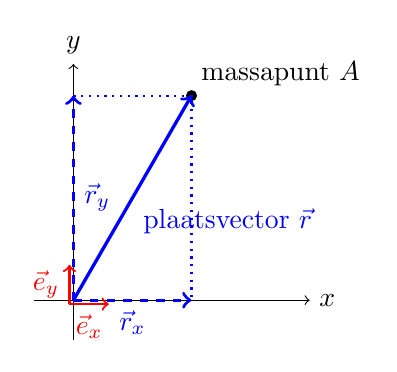
\begin{tikzpicture}
	
		\draw[->] (-0.5,0) -- (3,0) node[right] {$x$};
		\draw[->] (0,-0.5) -- (0,3) node[above] {$y$};
		\coordinate (O) at (0,0);

		\pgfmathsetmacro{\r}{3}       
		\pgfmathsetmacro{\ang}{60} 

		\coordinate (A) at (\ang :\r);

		\coordinate (X) at (\r*cos{\ang},0);
		\coordinate (Y) at (0,\r*sin{\ang});
	
		\fill (A) circle (2pt) node[above right] {massapunt $A$};
	
		\draw[->, very thick, blue] (O) -- (A) node[midway, below right] {plaatsvector $\vec{r}$};
		\draw[->, very thick, dashed, blue] (O) -- (X) node[midway, below] {$\vec{r}_x$};
		\draw[->, very thick, dashed, blue] (O) -- (Y) node[midway, right] {$\vec{r}_y$};
		\draw[thick, dotted, blue] (Y) -- (A) -- (X);
	
		\draw[->, thick, red, transform canvas={shift={(-0.05,-0.05)}}] (O) -- (0.5,0) node[midway, below] {$\vec{e}_x$};
		\draw[->, thick, red, transform canvas={shift={(-0.05,-0.05)}}] (O) -- (0,0.5) node[midway, left] {$\vec{e}_y$};
	\end{tikzpicture}
\end{image}
\captionof{figure}{De plaatsvector \(\vec{r}\)}
	

Als een puntmassa beweegt, verandert haar plaatsvector \(\vec{r}\).  
De beweging van een puntmassa wordt beschreven door een \textit{functie} die de \textbf{plaats} \(\vec{r}\) weergeeft in functie van de \textbf{tijd}. 
De \textbf{plaatsfunctie} \(\vec{r}\) = \(\vec{r}\)(t) geeft voor elk tijdstip \(t\) de positie \(\vec{r}\) waar de puntmassa zich bevindt. 
Op middelbaarniveau zijn dergelijke vectorfuncties ingewikkeld om te hanteren, daarom wordt geopteerd om te werken met de tijdsafhankelijke getalcomponenten \(x(t)\),\(y(t)\) en \(z(t)\).
Bij een ééndimensionale beweging is er slechts één daarvan nodig, namelijk \(x\). Dat is een getal, namelijk de positie op de enige coördinaatas
% \footnote{Een coördinaatas is een as van een cartesiaans assenstelsel, met een oorsprong en een ori\"entatie.} 
en $t$ is de variabele die symbool staat voor de tijd.
%\footnote{In de fysica gebruiken we de wiskunde als `taal' om de wetmatigheden van de natuur in uit te drukken. Wiskundige variabelen en objecten zoals functies krijgen nu een fysische betekenis. $x(t)$ is dus niets anders dan een functie $f(x)$ of $y(x)$ zoals je die in wiskunde kent. Alleen nemen wij nu niet voor de onafhankelijke variabele het symbool $x$ maar het symbool $t$ omdat deze symbool moet staan voor de tijd. En voor het symbool $f$ gebruiken wij nu het symbool $x$ omdat de beeldwaarden van de functie nu als betekenis een positie op een co\"ordinaatas hebben.}


De positie op een welbepaald tijdstip $t_1$ wordt genoteerd als 
%\footnote{Natuurlijk kan de index 1 ook vervangen worden door andere indices. Voorbeelden zijn $x_0=x(t_0)$ en $x_2=x(t_2)$.} komt de positie $x_1$ op de coördinaatas overeen volgens de formule
\begin{eqnarray*}
x_1=x(t_1)
\end{eqnarray*}

In onderstaande figuur zie je de tocht dat een zeilship aflegde. 
Op verschillende tijdstippen $t_0,t_1, t_2,\ldots$ wordt weergegeven waar het ship zich bevindt. 


% DIT KOMT UIT HET HANDBOEK --> VERVANGEN DOOR TIKZ VAN HET ZEILSCHIP 
% \begin{image}
% \includegraphics[width=0.45\textwidth]{Serway2p1(1)}
% $\qquad$   % hack 
% \includegraphics[width=0.45\textwidth]{Serway2p1(2)}
% \end{image}
% \captionof{figure}{Verschillende posities en de grafiek van de plaatsfunctie}


\pgfmathsetmacro{\at}{5}
\pgfmathsetmacro{\ax}{30}
\pgfmathsetmacro{\bt}{10}
\pgfmathsetmacro{\bx}{45}
\pgfmathsetmacro{\ct}{15}
\pgfmathsetmacro{\cx}{20}
\pgfmathsetmacro{\dt}{30}
\pgfmathsetmacro{\dx}{0}
\pgfmathsetmacro{\et}{45}
\pgfmathsetmacro{\ex}{-40}



% DE ZEILBOOT OP 1 LIJN ------------ % DE ZEILBOOT OP 1 LIJN ------ % DE ZEILBOOT OP 1 LIJN 
% DE ZEILBOOT OP 1 LIJN ------------ % DE ZEILBOOT OP 1 LIJN ------ % DE ZEILBOOT OP 1 LIJN
% DE ZEILBOOT OP 1 LIJN ------------ % DE ZEILBOOT OP 1 LIJN ------ % DE ZEILBOOT OP 1 LIJN
\begin{image}[0.5\textwidth]
\begin{tikzpicture}
\begin{axis}[
	axis x line=bottom,
	axis y line=none,       % no vertical axis
	axis line style={->},
	xmin=-50, xmax=55,    % position axis
	ymin=-1, ymax=3,        % enough room for icons + labels
	width=14cm, height=4cm,
	xlabel={Positie--as (in meter)},
	xtick={-50,-40,...,50},
	xticklabel={\SI[round-precision=0, round-mode=places]{\tick}{m}}, % gaf eerst in beduidende cijfers 
	% yticklabel={\SI[round-precision=0, round-mode=places]{\tick}{m}},
]

% --- Ships at given positions ---
\node[opacity=0.2,scale=1,xscale=-1]  (ship1) at (axis cs:\ax,0.5)  {\includegraphics[width=1cm]{schip_icoon}};
\node[opacity=0.5,scale=1,xscale=0.7] (ship2) at (axis cs:\bx,0.5)  {\includegraphics[width=1cm]{schip_icoon}};
\node[opacity=0.7]                     (ship3) at (axis cs:\cx,0.5) {\includegraphics[width=1cm]{schip_icoon}};
\node[]                                (ship4) at (axis cs:\dx,0.5) {\includegraphics[width=1cm]{schip_icoon}};
\node[]                                (ship5) at (axis cs:\ex,0.5) {\includegraphics[width=1cm]{schip_icoon}};

% --- Time labels above ships ---
\node[draw, rectangle, inner sep=1pt] (t1) at (axis cs:\ax,2.2) {\small $t_1=\SI{\at}{\second}$};
\node[draw, rectangle, inner sep=1pt] (t2) at (axis cs:\bx,2.2) {\small $t_2=\SI{\bt}{\second}$};
\node[draw, rectangle, inner sep=1pt] (t3) at (axis cs:\cx,2.2) {\small $t_3=\SI{\ct}{\second}$};
\node[draw, rectangle, inner sep=1pt] (t4) at (axis cs:\dx,2.2) {\small $t_4=\SI{\dt}{\second}$};
\node[draw, rectangle, inner sep=1pt] (t5) at (axis cs:\ex,2.2) {\small $t_5=\SI{\et}{\second}$};

\end{axis}
\end{tikzpicture}
\end{image}
\captionof{figure}{De positie van de zeilboot voor elke tijd \(t\)}


In de natuurkunde is \textbf{tijd een dimensie}.\footnote{Einstaan gaf een beschrijving voor de zwaartekracht in de \textit{4-dimensionale ruimte-tijd}.}
In bovenstaande figuur wordt bovenaan aangegeven boven elke zeilboot op welk tijdstip de boot daar was waargenomen. 
Zo bevindt de boot zich op \(t_3 = \SI{15}{s}\) op de positie \(\SI{20}{meter}\). 
Deze informatie over de tijd kan worden weergegeven op een tijd-as. 




% ZEILBOOT OP TIJDSAS ------ ZEILBOOT OP TIJDSAS ------ ZEILBOOT OP TIJDSAS 
% ZEILBOOT OP TIJDSAS ------ ZEILBOOT OP TIJDSAS ------ ZEILBOOT OP TIJDSAS 
% ZEILBOOT OP TIJDSAS ------ ZEILBOOT OP TIJDSAS ------ ZEILBOOT OP TIJDSAS 

\begin{image}[0.5\textwidth]
\begin{tikzpicture}
	\begin{axis}[
		axis x line=bottom,
		axis y line=left,
		axis line style={->},
		xlabel={tijd (in seconden)},
		ylabel={positie (in meter)},
		xmin=0, xmax=50,
		ymin=-50, ymax=65,
		xtick={0,10,...,50},
		ytick={-50,-40,...,50}, % keep normal marks
		xticklabel={\SI[round-precision=0, round-mode=places]{\tick}{s}},
		yticklabel={\SI[round-precision=0, round-mode=places]{\tick}{m}},
		grid=both,
		width=15cm, height=10cm,
	]
	
	% --- The position–time curve ---
	% \addplot[blue, thick] coordinates{
	% 	(\at,\ax)
	% 	(\bt,\bx)
	% 	(\ct,\cx)
	% 	(\dt,\dx)
	% 	(\et,\ex)
	% };
	
	% --- Ships as markers at data points ---
	\node[] at (axis cs:\at,\ax) {\includegraphics[width=1cm]{schip_icoon}};
	\node[] at (axis cs:\bt,\bx) {\includegraphics[width=1cm]{schip_icoon}};
	\node[] at (axis cs:\ct,\cx) {\includegraphics[width=1cm]{schip_icoon}};
	\node[] at (axis cs:\dt,\dx) {\includegraphics[width=1cm]{schip_icoon}};
	\node[] at (axis cs:\et,\ex) {\includegraphics[width=1cm]{schip_icoon}};
	
	% --- Time labels above each ship ---
	\node[draw, rectangle, inner sep=1pt] at (axis cs:\at,\ax+10) {\small $t_1=\SI{\at}{\second}$};
	\node[draw, rectangle, inner sep=1pt] at (axis cs:\bt,\bx+10) {\small $t_2=\SI{\bt}{\second}$};
	\node[draw, rectangle, inner sep=1pt] at (axis cs:\ct,\cx+10) {\small $t_3=\SI{\ct}{\second}$};
	\node[draw, rectangle, inner sep=1pt] at (axis cs:\dt,\dx+10) {\small $t_4=\SI{\dt}{\second}$};
	\node[draw, rectangle, inner sep=1pt] at (axis cs:\et,\ex+10) {\small $t_5=\SI{\et}{\second}$};
	
	\end{axis}
	\end{tikzpicture}
\end{image}
\captionof{figure}{De positie van de zeilboot met een tijd-as}


Er zit \textbf{geen} extra informatie in bovenstaande figuur! 
We hebben enkel de tijdsdimensie uitgezet op een horizontale-as. 
Als je nu ijverig natuurkunde aan het studeren bent, kan je 'de positie' van dit blad papier onderzoeken. 
Dit blad ligt stil op je bureau en je probeert te begrijpen wat er uitgelegd wordt. 
Echter, als je de tijdsdimensie in rekening brengt, verandert de positie je blad wel\footnote{Want terwijl je dit aan het lezen bent staat de tijd natuurlijk niet stil...\footnotemark}
\footnotetext{Je blad beweegt zich -eerder saai- constant voort op de tijdsdimensie. Het is echter mogelijk -in de relativiteitstheorie- om ook op meer interessantere manieren op de tijd-as te bewegen.\footnotemark}
\footnotetext{Aangezien je enkel constant op de tijd-as kan voortbewegen, en dus niet terug kan, lijkt het aangewezen om je tijd goed te benutten. Bijvoorbeeld door wat natuurkunde te leren.}

De positie van de zeilboot is enkel weergegeven voor een aantal specifieke momenten \(t_i\). In bovenstaande figuur kan voor elke moment \(t\) de positie worden weergegeven, op die manier bekom je de \textbf{plaatsfunctie}. 


\begin{image}[0.5\textwidth]
\begin{tikzpicture}
	\begin{axis}[
		axis x line=bottom,
		axis y line=left,
		axis line style={->},
		xlabel={tijd (in seconden)},
		ylabel={positie (in meter)},
		xmin=0, xmax=50,
		ymin=-50, ymax=65,
		xtick={0,10,...,50},
		ytick={-50,-40,...,50}, % keep normal marks
		xticklabel={\SI[round-precision=0, round-mode=places]{\tick}{s}},
		yticklabel={\SI[round-precision=0, round-mode=places]{\tick}{m}},
		grid=both,
		width=15cm, height=10cm,
	]
	
	% --- The position–time curve ---
	\addplot[blue, thick, smooth, tension=0.5] coordinates{
		(\at,\ax)
		(\bt,\bx)
		(\ct,\cx)
		(\dt,\dx)
		(\et,\ex)
	};
	
	% --- Ships as markers at data points ---
	\node[] at (axis cs:\at,\ax) {\includegraphics[width=1cm]{schip_icoon}};
	\node[] at (axis cs:\bt,\bx) {\includegraphics[width=1cm]{schip_icoon}};
	\node[] at (axis cs:\ct,\cx) {\includegraphics[width=1cm]{schip_icoon}};
	\node[] at (axis cs:\dt,\dx) {\includegraphics[width=1cm]{schip_icoon}};
	\node[] at (axis cs:\et,\ex) {\includegraphics[width=1cm]{schip_icoon}};
	
	% --- Time labels above each ship ---
	\node[draw, rectangle, inner sep=1pt] at (axis cs:\at,\ax+10) {\small $t_1=\SI{\at}{\second}$};
	\node[draw, rectangle, inner sep=1pt] at (axis cs:\bt,\bx+10) {\small $t_2=\SI{\bt}{\second}$};
	\node[draw, rectangle, inner sep=1pt] at (axis cs:\ct,\cx+10) {\small $t_3=\SI{\ct}{\second}$};
	\node[draw, rectangle, inner sep=1pt] at (axis cs:\dt,\dx+10) {\small $t_4=\SI{\dt}{\second}$};
	\node[draw, rectangle, inner sep=1pt] at (axis cs:\et,\ex+10) {\small $t_5=\SI{\et}{\second}$};
	
	\end{axis}
\end{tikzpicture}
\end{image}	


\begin{definition} 
	De \textbf{plaatsfunctie} \(\vec{x}(t)\) geeft voor elke moment \(t\) de positievector \(x\). 
	In één dimensie is \(\vec{x}\) een scalar en is de plaatsfuncie een grafiek waarop horizontaal de tijd wordt weergegeven en verticaal de positie. 

\begin{image}[0.3\textwidth]
	\begin{tikzpicture}
		\begin{axis}[
			axis lines=middle,
			xlabel={tijd \(t\)}, ylabel={positie \(\vec{x}\)},
			grid=both,
			width=10cm, height=6cm,
			xmin=0, xmax=6, ymin=0, ymax=6,
			xtick=\empty,
			ytick=\empty,
			clip=false,
		]
			Coordinates
			\addplot[
				only marks,
				mark=*,
				mark size=2pt,
				color=red
			] coordinates {
				(1,3) (3,2)
			};
	
			% Interpolating function through the points
			\addplot[
				smooth,
				thick,
				color=blue
			] coordinates {
				(0,1) (1,3) (3,2) (4,3) (6,4)
			};

		% Project points (example: first and last points)
		\draw[dashed] (axis cs:1,3) -- (axis cs:1,0) node[below]{$t_a$};
		\draw[dashed] (axis cs:1,3) -- (axis cs:0,3) node[left]{$x_a$};
		\draw[dashed] (axis cs:3,2) -- (axis cs:3,0) node[below]{$t_b$};
		\draw[dashed] (axis cs:3,2) -- (axis cs:0,2) node[left]{$x_b$};

		\end{axis}
	\end{tikzpicture}

\end{image}
\end{definition}



% WE GAAN SEBIET DE PLAATSVFUCTIE HERNEMEN EN HIER DELTA X EN T OPZETTEN --> KAN DEZE FIGUUR VERVANGEN 
% In onderstaande figuur zie je voor een bepaalde 1D beweging ook de begin- en eindplaatsvectoren met hun plaatscoördinaten die dan in een grafiek als functie van de tijd wordt weergegeven.

% \begin{image}
% \includegraphics[width=0.8\textwidth]{positiemetgrafiek}
% \end{image}
% \captionof{figure}{Links het verplaatsend voorwerp met begin- en eindpositie. Rechts de grafiek van \(x(t)\).}


\newpage %heel tijdelijk


De \textbf{verplaatsing} tussen $t_1$ en $t_2$ is het verschil in positie tussen de twee tijdstippen $t_1$ en $t_2$, genoteerd met een $\Delta$\(\vec{r}\) (Delta, een Griekse hoofdletter D  van het Engelse 'displacement' of het Franse 'déplacement').

\begin{definition}
De \textbf{verplaatsing} \(\Delta \vec{r}\) is het verschil tussen twee posities:
\[
\Delta \vec{r} = \vec{r}_2 - \vec{r}_1
\]

\tikzset{>={latex[scale=1.2]}}

\begin{image}[0.3\textwidth]
	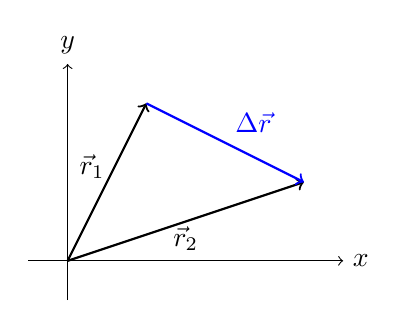
\begin{tikzpicture}
		
		\draw[->] (-0.5,0) -- (3.5,0) node[right] {$x$};
		\draw[->] (0,-0.5) -- (0,2.5) node[above] {$y$};
		
		\coordinate (X) at (1,2);
		\coordinate (Y) at (3,1);
		
		% \fill (X) circle (2pt) node[above] {};
		% \fill (Y) circle (2pt) node[above right] {};
		
		\draw[->, thick] (0,0) -- (X) node[pos= 0.6, left] {$\vec{r}_1$};
		\draw[->, thick] (0,0) -- (Y) node[midway, below, yshift=2pt] {$\vec{r}_2$};
		\draw[->, thick, blue] (X) -- (Y) node[midway, above right] { $\Delta \vec{r}$};

	\end{tikzpicture}
\end{image}
\end{definition}
% TODO: opmerking toevoegen dat de natatie $\Delta$ *erg* slecht is, omdat ze de indices 1 en 2 niet bevat!





Voor ééndimensionale bewegingen is de verplaatsing eenvoudig scalair te berekenen met: $\Delta x$ = $x_{eind}-x_{begin}$.
De verplaatsing van de zeilboot tussen de tijdstippen $t_0$ en $t_1$ is gelijk aan \( \Delta x = x_1-x_0 = \SI{45}{meter} - \SI{30}{meter} = \SI{15}{meter}\)  en is de verplaatsing tussen de tijdstippen $t_2$ en $t_4$ gelijk aan \(\Delta x=x_4-x_2=\SI{-40}{meter} - \SI{0}{meter} = \SI{-40}{meter}\). Deze laatste verplaatsing is negatief, wat aangeeft dat de zeilboot netto naar achteren is bewogen -- tegengesteld aan de zin van de gekozen as.

Op de plaatsfunctie kan de verplaatsing eenvoudig afgelezen worden: 

\begin{image}
\begin{tikzpicture}
	\begin{axis}[
		axis lines=middle,
		xlabel={tijd \(t\)}, ylabel={positie \(\vec{x}\)},
		grid=both,
		width=10cm, height=6cm,
		xmin=0, xmax=6, ymin=0, ymax=6,
		xtick=\empty,
		ytick=\empty,
		clip=false,
	]
		Coordinates
		\addplot[
			only marks,
			mark=*,
			mark size=2pt,
			color=red
		] coordinates {
			(1,3) (3,2)
		};

		% Interpolating function through the points
		\addplot[
			smooth,
			thick,
			color=blue
		] coordinates {
			(0,1) (1,3) (3,2) (4,3) (6,4)
		};

	% Project points (example: first and last points)
	\draw[dashed] (axis cs:1,3) -- (axis cs:1,0) node[below](tijda) {$t_a$};
	\draw[dashed] (axis cs:1,3) -- (axis cs:0,3) node[left] (positiea) {$x_a$};
	\draw[dashed] (axis cs:3,2) -- (axis cs:3,0) node[below] (tijdb) {$t_b$};
	\draw[dashed] (axis cs:3,2) -- (axis cs:0,2) node[left](positieb) {$x_b$};

	\draw[dashed] (positiea) -- (positieb);
	\draw[<->, dashed] (tijda) -- (tijdb) node[midway, fill=white]{\(\Delta t\)};
	\end{axis}
\end{tikzpicture}
\end{image}

% DEZE WERKT NIET IN DE HTML MOMENTEEL... 
% \begin{quickquestion*}
% 	Bereken de verplaatsing \(\Delta x = x_4 - x_1\) van de zeilboot en duidt deze verplaatsing aan op de grafiek.  
% \end{quickquestion*}


Let op, de verplaatsing hoeft niet noodzakelijk gelijk te zijn aan de \emph{afgelegde weg} tussen de twee bijbehorende tijdstippen. Als je een rondje hebt gelopen op de atletiekpiste en terug aan start staat is je (netto) verplaatsing nul, maar heb je wel degelijk afstand afgelegd.

Samengevat voor ééndimensionale bewegingen:





% OMGEZET NAAR TABULARS
% \begin{image}
% \includegraphics[width=0.8\textwidth]{positieverplaatsing1D}

% \end{image}




% \begin{tabular}{p{4cm}|p{4cm}}
% 	\textbf{Vectoriële notatie} & \textbf{Scalaire notatie} \\ \midrule
% 	Positie op moment $t$: & \\
% 	$\vecx(t) = x(t) \cdot \ehatx = x \cdot \ehatx$ & $x(t) = x$ \\
% 	& (kan negatief zijn) \\ \midrule
% 	Verplaatsing op tijdsinterval $\deltat = t_2 - t_1$: & \\
% 	$\Delta\vecx = \vecxtwo - \vecxone$ & $\deltax = x_2 - x_1$ \\
% 	$= x_2 \cdot \ehatx - x_1 \cdot \ehatx = (x_2 - x_1) \cdot \ehatx = \deltax \cdot \ehatx$ & (kan negatief zijn bij verplaatsing tegen de zin van de $x$-as) \\ \midrule
% 	Afgelegde weg op moment $t$: & \\
% 	$\left| \vecx(t) \right|$ & $s(t)$ \\
% 	(afgelegde verplaatsing) & (kan niet negatief zijn, zie wiskunde) \\
% \end{tabular}

% \begin{center}
% 	\begin{tabular}{p{5cm} c c}
% 		& Vectoriële notatie                                   & Scalaire notatie        \\ [10pt]
% 		\cline{2-3}
% 		Positie op moment \(t\):                               & $\vec{x}_t = x(t)\cdot\vec{e}_x = x\cdot\vec{e}_x $  & $x(t) = x$              \\ [10pt]
% 		Verplaatsing op \newline tijdsinterval $\Delta t = t_2 - t_1 $: & $\Delta\vec{x} = \vec{x}_2 - \vec{x}_1$              & $\Delta x = x_2 - x_1 $ \\ [10pt]
% 		Afgelegde weg op moment t:                             &  $\diagup$                                           & $s(t)$
% 	\end{tabular}
% \end{center}




% SCALAIR EN VECTORIEEL NOG OMDRAAIEN
\fbox{
\begin{tabular}{p{5cm} >{\centering\arraybackslash}p{5cm} >{\centering\arraybackslash\arraybackslash}p{5cm}}
																		& Vectoriële notatie                                            & Scalaire notatie        \\ [4pt]
	% \cline{2-3}\noalign{\vskip 8pt}
	Positie op moment \(t\):                                            & \fbox{$\vec{x}_t = x(t)\cdot\vec{e}_x = x\cdot\vec{e}_x $ }   & \fbox{$x(t) = x$}  \newline \tiny{(kan negatief zijn)}             \\ [15pt]
	Verplaatsing op het \newline tijdsinterval $\Delta t = t_2 - t_1 $: & \fbox{$\Delta\vec{x} = \vec{x}_2 - \vec{x}_1$} \newline \tiny{$\Delta x \cdot \vec{e}_x = (x_2-x_1)\cdot \vec{e}_x = x_2\cdot\vec{e}_x - x_1\cdot\vec{e}_x$ } & \fbox{$\Delta x = x_2 - x_1 $} \newline \tiny{(kan negatief zijn bij een verplaatsing tegen de zin van de \(x\)-as.)}\\ [20pt]
	Afgelegde weg op moment t:                                          &  $\diagup$                                                    & $s(t)$ \newline \tiny{kan negatief zijn; zie wiskunde}
\end{tabular}
}
	



Voor tweedimensionale bewegingen worden de begrippen positie, verplaatsing en afgelegde weg complexer.

\begin{image}
\includegraphics[width=0.8\textwidth]{positie2D}

\end{image}

\begin{image}
\includegraphics[width=0.8\textwidth]{verplaatsing2D}

\end{image}


Wanneer een voorwerp beweegt, doorloopt het meerdere posities. De verbindingslijn van al deze gepasseerde posities, noemt men de \textbf{baan} van de beweging. 
Een ééndimensionale beweging heeft een rechte baan. Een tweedimensionale is doorgaans krom en kan meerdere vormen hebben zoals cirkelvormig, paraboolvormig, ellipsvormig,...
Soms is men geïnteresseerd in een \textbf{baanvergelijking} waarin men de afhankelijkheid tussen x en y wiskundig neerschrijft.
Indien de functies \(x(t)\) en \(y(t)\) gekend zijn, kan soms een (expliciete) baanvergelijking bekomen worden door één voorschrift uit te werken naar \(t\) en dit vervolgens te substitueren in de andere vergelijking.

\begin{image}
\includegraphics[width=0.8\textwidth]{vbBaanvergelijking}

\end{image}
	
\end{document}





% DIT WAS EEN TEST OM DIE SINUS UIT HET HANDBOEK NA TE MAKEN 
% \begin{image}
% 	\begin{tikzpicture}
% 	\begin{axis}[
% 		axis x line=bottom,
% 		axis y line=left,
% 		xlabel={$x$}, ylabel={$y$},
% 		xmin=0, xmax=50,              % x-axis 0 to 50
% 		ymin=-45, ymax=60,            % y-axis -60 to 60
% 		xtick={0,10,...,50},          % x ticks every 10
% 		ytick={-60,-50,...,60},       % y ticks every 10
% 		grid=both,
% 		width=12cm, height=6cm,
% 		samples=200,
% 		domain=0:50,
% 		axis line style={->},         % arrows at ends
% 		% scale y visually double the x
% 		x=0.2cm,                      % compress x
% 		y=0.1cm,                      % stretch y
% 		enlarge y limits=0.05,
% 	]
% 		% scaled sine function to fit -60..60
% 		\addplot[blue, thick] {60*sin(deg((pi/50)*x + pi/4))};
% 	\end{axis}
% 	\end{tikzpicture}
% \end{image}
